\documentclass[a4paper, 12pt]{article} % Fuente 12pt
\usepackage[T1]{fontenc}
\usepackage{hyperref}
\usepackage[left=3cm, right=3cm, top=3.5cm, bottom=3.5cm]{geometry} % Márgenes recomendados
\usepackage{times} % Fuente Times New Romans
\usepackage[spanish, english]{babel} 
\usepackage[style=ieee, backend=bibtex,citestyle=numeric-comp]{biblatex} % Bibliografía en formato IEEE
\usepackage{sectsty}
\usepackage{cover/cover}
\usepackage{graphicx}
\usepackage{subfig}
\graphicspath{ {images/} } % Directorio imágenes
\usepackage{listings} % Formateo código
\lstset{
  basicstyle=\ttfamily,
  columns=fullflexible,
  frame=single,
  breaklines=true,
  postbreak=\mbox{\textcolor{black}{$\hookrightarrow$}\space},
}
\usepackage{scrextend}
\usepackage{longtable}
\usepackage{pgfplots} % Graficas de barras
\usepackage{pgf-pie} % Graficas de tartas
\usepackage{multirow} % multiples filas en las tablas
\usepackage[utf8]{inputenc}
% Lista de acronimos
\usepackage[acronym]{glossaries}
% List of acronyms
\newacronym{CTF}{CTF}{Capture The Flag}
\newacronym{htb}{HTB}{Hack The Box}
\newacronym{ftp}{FTP}{File Transfer Protocol}
\newacronym{ssh}{SSH}{Secure Shell}
\newacronym{tcp}{TCP}{Transmission Control Protocol}
\newacronym{http}{HTTP}{Hypertext Transfer Protocol}
\newacronym{url}{URL}{Uniform Resource Locator}
\newacronym{ip}{IP}{Internet Protocol}
\newacronym{ids}{IDS}{Intrusion Detection System}
\newacronym{dns}{DNS}{Domain Name System}
\newacronym{uri}{URI}{Uniform Resource Identifier}
\makeglossaries
\sectionfont{\MakeUppercase} % Secciones en mayúsculas
\bibliography{sections/Bibliography.bib}

\Director{Luis Alfonso Rodríguez De Trio y Pérez}
\Lugar{Madrid} 
\Master{Máster en Seguridad Informática y Hacking Ético} 
\Trabajo{TRABAJO FIN DE MÁSTER} 

\author{Víctor Nieves Sánchez}
\date{Octubre de 2021}
\title{Resolución y explicación de \textit{Cap} y \textit{Seal} (\acrshort{HTB})}

\begin{document}
\maketitle
\null
\newpage
\begin{otherlanguage}{spanish}

    \pagenumbering{roman} % Numeración romana hasta la primera sección

    %\begin{otherlanguage}{spanish}
    %    \renewcommand{\spanishabstractname}{Agradecimientos}
    %    \begin{abstract}
    %        % Si lees esto es que eres o muy listo, o muy vago como para intentarlo.
% La solución es: 
%   1) Metadata
%   2) Comentario
%   3) Base64
%   4) JWT Decoder
%   5) Binary Decoder
%   6) Agradecimientos
%
%   No todo va a ser CTFs y hacer TFGs/TFMs ...

\begin{lstlisting}[language=html]
    <img src="./images/?.jpeg" alt="Let's play a game!" onerror=alert('WTF')>
\end{lstlisting}
    %    \end{abstract}
    %\end{otherlanguage}

    \newpage
    \tableofcontents

    \newpage
    \listoffigures

    \newpage
    \renewcommand{\listtablename}{Lista de Tablas}
    \listoftables

    \newpage
    \lstlistoflistings

    \newpage
    \printglossary[type=\acronymtype]

    \newpage
    \begin{abstract}
        \normalsize
        \# TODO

\textbf{Keywords:} Hacking, Ciberseguridad, \acrlong{HTB}, \acrshort{CTF}, \acrlong{ceh}\ldots

    \end{abstract}

    \newpage
    \renewcommand{\spanishabstractname}{Abstract}
    \begin{abstract}
        \normalsize
        In the technology industry, cybersecurity is very important.  Companies are increasingly focused on ensuring that their various applications, projects and services are secure.  They are even starting to adapt their solutions to technologies that guarantee greater security and robustness, such as Blockchian technology.\\

On the other hand, companies must protect the information security, guaranteeing the confidentiality, availability and integrity of the information. This problem is often linked to data protection regulations, such as the \acrshort{gdpr}, which is why the idea of a "\acrlong{ssi}" is becoming increasingly popular.  \acrfull{ssi} is the concept that individuals or organizations have the sole and exclusive ownership of their digital identities, and are the ones who control how their personal data is shared and used.\\

Alastria, a consortium promoting the digital economy through the development of decentralized registration technologies such as Blockchain, has defined a digital identity model called \textit{Alastria ID}. The \textit{Alastria ID} project is deployed as one of the basic applications of the blockchain infrastructure promoted by the consortium within its platform.  This technological proposal of digital identity in blockchain aims to provide an infrastructure and development framework to carry out \acrfull{ssi} projects, with full legal validity in the euro area.\\

The fact that a company uses Blockchain technology does not mean that it is free of security problems and vulnerabilities.  As these are new technologies, there are still not many standards, there are no robust implementations, and a small failure can cause a security gap, and the impact this can have on a \acrlong{ssi} model can be critical to the ecosystem.\\

The objective of this work is multiple. The concept of \acrfull{ssi} has been studied, as well as the implementation of Alastria called \textit{Alastria ID} and other implementations and solutions that exist today. On the other hand, a study of the \textit{Alastria ID} implementation has been carried out from the point of view of security, auditing the Smart Contracts designed in the \acrshort{mvp}1 and the library that facilitates its use. Finally, a \acrlong{poc} has been created for one of the vulnerabilities found during the analysis phase and its criticality and impact has been evaluated.\\

\textbf{Keywords:} Blockchain, Alastria, \acrlong{ssi}, Ethereum, Quorum, Solidity, Smart Contracts, Hacking, Cybersecurity, Information Security, Audit\ldots


    \end{abstract}
    \newpage
    \pagenumbering{arabic} % Numeración árabe en la primera sección

    \section{Introducción}
    voy a resolver varias máquinas
    - contexto
    - motivacion
    - objetivos
    - estructura del documento

    \newpage
    \section{Estado del Arte}
    
    \subsection{Hacking Ético}
    El programa \textit{\acrfull{ceh}} define el hacking ético como:

\begin{quote}
    \textit{la práctica de emplear conocimientos informáticos y de redes para ayudar a las organizaciones a probar la seguridad de su red en busca de posibles lagunas y vulnerabilidades}
\end{quote}

Los hackers éticos informan de todas las vulnerabilidades al propietario del sistema y de la red para que se corrijan, aumentando así la seguridad del sistema de información de una organización. El hacking ético implica el uso de herramientas, trucos y técnicas de hacking típicamente utilizadas por un atacante para verificar la existencia de vulnerabilidades explotables en la seguridad del sistema.\\

Hoy en día, el término \textit{hacking} está estrechamente asociado a actividades ilegales y poco éticas. Se sigue debatiendo si el hacking puede ser ético o no, dado que el acceso no autorizado a cualquier sistema es un delito. Por eso es importante destacar las siguientes definiciones:

\begin{itemize}
    \item El término "\textbf{hacker}" se refiere a una persona que disfruta aprendiendo los detalles de los sistemas informáticos y ampliando sus capacidades.
    \item El verbo "\textbf{hackear}" describe el rápido desarrollo de nuevos programas o la ingeniería inversa del software existente para hacerlo mejor o más eficiente de formas nuevas e innovadoras.
    \item Los términos "\textbf{cracker}" y "\textbf{atacante}" se refieren a las personas que emplean sus habilidades de hacking con fines ofensivos.
    \item El término "\textbf{hacker ético}" se refiere a los profesionales de la seguridad que emplean sus habilidades de hacking con fines defensivos.
\end{itemize}

En la actualidad, el hacking ético es necesario porque permite a las organizaciones contrarrestar los ataques de los hackers malintencionados, anticipando los métodos que utilizan para entrar en los sistemas. El hacking ético ayuda a predecir con antelación las distintas vulnerabilidades posibles y a rectificarlas antes de sufrir ningún tipo de ataque externo.


\subsubsection{Tipos de Hacker}

Aunque solo existe una tipología de hacking que sea ético, es interesante explicar los tipos de hacker que hay.

\begin{itemize}
    \item \textbf{Sombrero negro} o \textbf{Black hat}: son aquellos que tiene los conocimientos necesarios para romper la seguridad de un sistema o programa, o para crear virus y los utiliza con malas intenciones.
    \item \textbf{Sombrero blanco} o \textbf{White hat}: cuentan con los conocimientos necesarios para saltarse la seguridad de un sistema o crear virus, pero los usan para hacer el bien ayudando a mejorar la seguridad de organizaciones y empresas.
    \item \textbf{Sombrero gris} o \textbf{Grey hat}: son aquellos que tienen una ética ambigua. Es decir, tienen los conocimientos de los \textit{blacks hats} y los utilizan para entrar en sistemas pero no explotan las vulnerabilidades con fines maliciosos.
\end{itemize}

También existen otros términos para definir a los hackers, como los \textbf{\textit{script kiddies}}, los \textbf{\textit{hacktivistas}} o los equipos/grupos de hackers (\textbf{\textit{hacker teams}}).

\subsubsection{Habilidades de un Hacker Ético}

Es esencial que un hacker ético adquiera los conocimientos y habilidades necesarios para convertirse en un hacker experto y utilizar estos conocimientos de forma lícita. Algunas de esas habilidades son:

\begin{itemize}
    \item \textbf{Habilidades técnicas}:
          \begin{itemize}
              \item Conocimiento profundo de los principales entornos operativos, como \textit{Windows}, \textit{Linux/Unix} y \textit{Mac OS}.
              \item Conocimiento profundo de los conceptos y tecnologías de redes, y del hardware y software relacionados.
              \item Conocimiento de las áreas de seguridad y temas relacionados.
              \item Alto conocimiento técnico de cómo lanzar ataques sofisticados.
          \end{itemize}
    \item \textbf{Habilidades no técnicas}:
          \begin{itemize}
              \item La capacidad de aprender y adaptar rápidamente las nuevas tecnologías.
              \item Una fuerte ética de trabajo y buenas habilidades de comunicación y resolución de problemas.
              \item Compromiso con las políticas de seguridad de la organización.
              \item Conocimiento de las normas y leyes locales.
          \end{itemize}
\end{itemize}

    \subsection{\acrlong{HTB}}
    \acrfull{HTB}\cite{htb} (figura \ref{fig:htb-logo}) es una plataforma online gratuita que une a cientos de miles de hackers. En el núcleo de \acrshort{HTB} hay una red de máquinas vulnerables listas para ser atacadas y para que se practiquen las habilidades de ciberseguridad, de forma totalmente legal. El objetivo es realizar un \acrshort{CTF}, es decir, conseguir ser root para demostrar que has conseguido el control total sobre la máquina.\\

\begin{figure}[h]
    \centering
    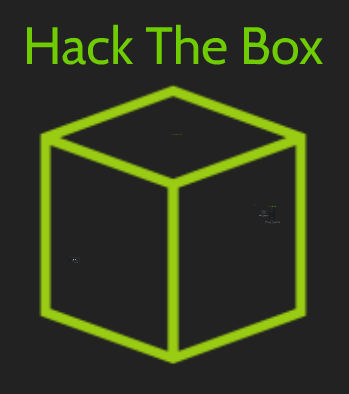
\includegraphics[width=0.40\textwidth]{images/sections/stateOfTheArt/htb-logo.png}
    \caption{Logo de \textit{\acrshort{HTB}}}
    \label{fig:htb-logo}
\end{figure}

En \acrshort{HTB} hay distintos desafíos, como \textit{machines}, \textit{challenges}, \textit{tracks} y más, cada uno con distintos niveles de dificultad (``\textit{easy}``, ``\textit{medium}``, ``\textit{hard}`` e ``\textit{insane}``), además de un \textit{Starting Point} para personas que se enfrenten por primera vez a este tipo de desafíos. Cada desafío proporciona una serie de puntos que sirven para escalar en el \textit{ranking} global.

\acrshort{HTB} tiene una subscripción de pago que te permite acceder a las máquinas retiradas, además de proporcionarte más características, como laboratorios VIP o acceso a \textit{write-ups} oficiales.\\

A continuación se mencionan los principales laboratorios en \acrshort{HTB}.

\subsubsection{Challenges}
Los desafíos (\textit{challenges}) están categorizados por su temática, como se muestra en la figura \ref{fig:htb-challenges}. Cada desafío tiene una dificultad, y se centra en resolver el desafío para encontrar el flag pertinente.

\begin{figure}[h]
    \centering
    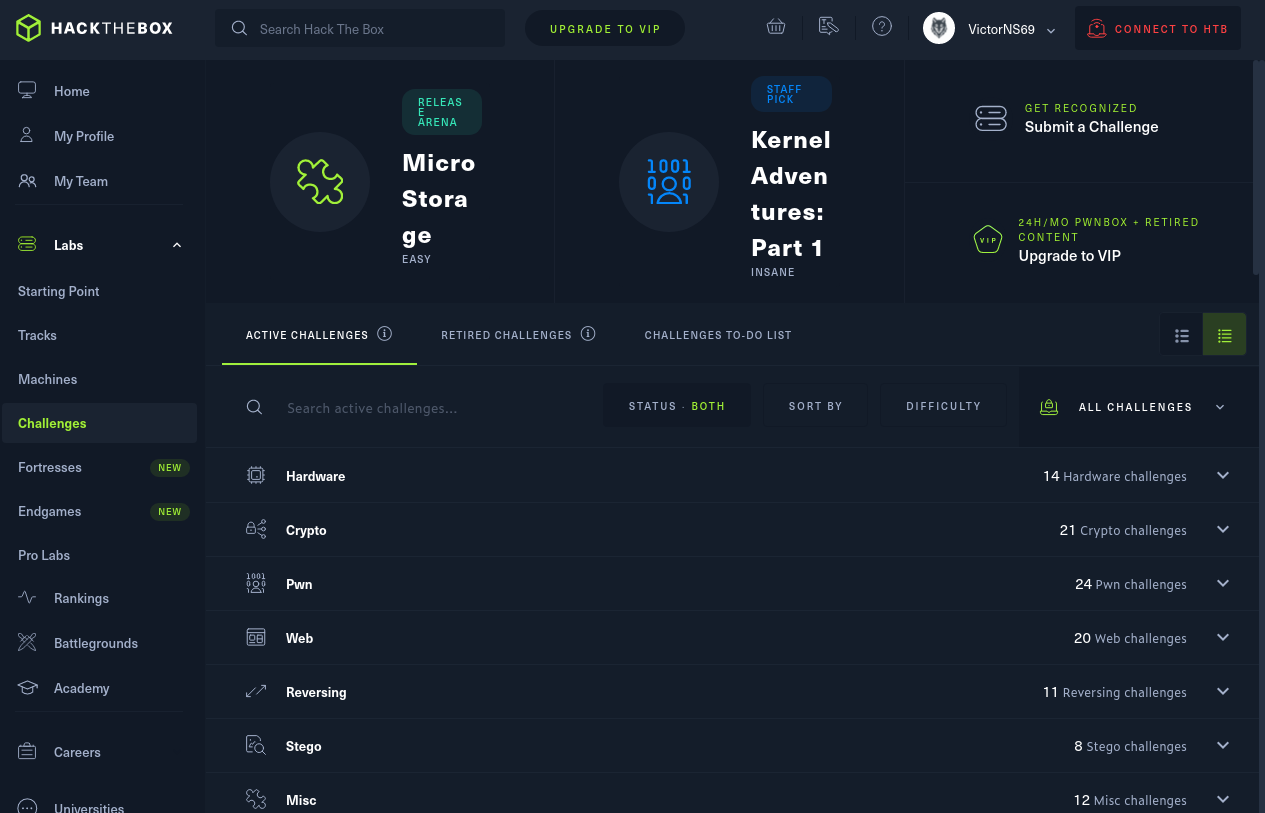
\includegraphics[width=0.7\textwidth]{images/sections/stateOfTheArt/htb-challenges.png}
    \caption{Tipos de \textit{challenges} en \textit{\acrshort{HTB}}}
    \label{fig:htb-challenges}
\end{figure}

\subsubsection{Machines}
Las máquinas (\textit{machines}) intentan simular en mayor o menor medida a un servidor real, con páginas web, servicios de administración como \acrshort{ssh} o \textit{telnet}, descarga y subida de ficheros a través de \acrshort{ftp}, servidores de dominio Window, etc. Para poder conseguir ser root se tendrán que usar técnicas de escalada de privilegios, esteganografía, fuerza bruta, exploits, análisis de código y cualquier conocimiento del mundo de la ciberseguridad. En la figura \ref{fig:htb-machines} se pueden ver las máquinas disponibles a fecha de la realización de este trabajo. Las máquinas van desapareciendo y van naciendo máquinas nuevas con el paso del tiempo.\\

\begin{figure}[h]
    \centering
    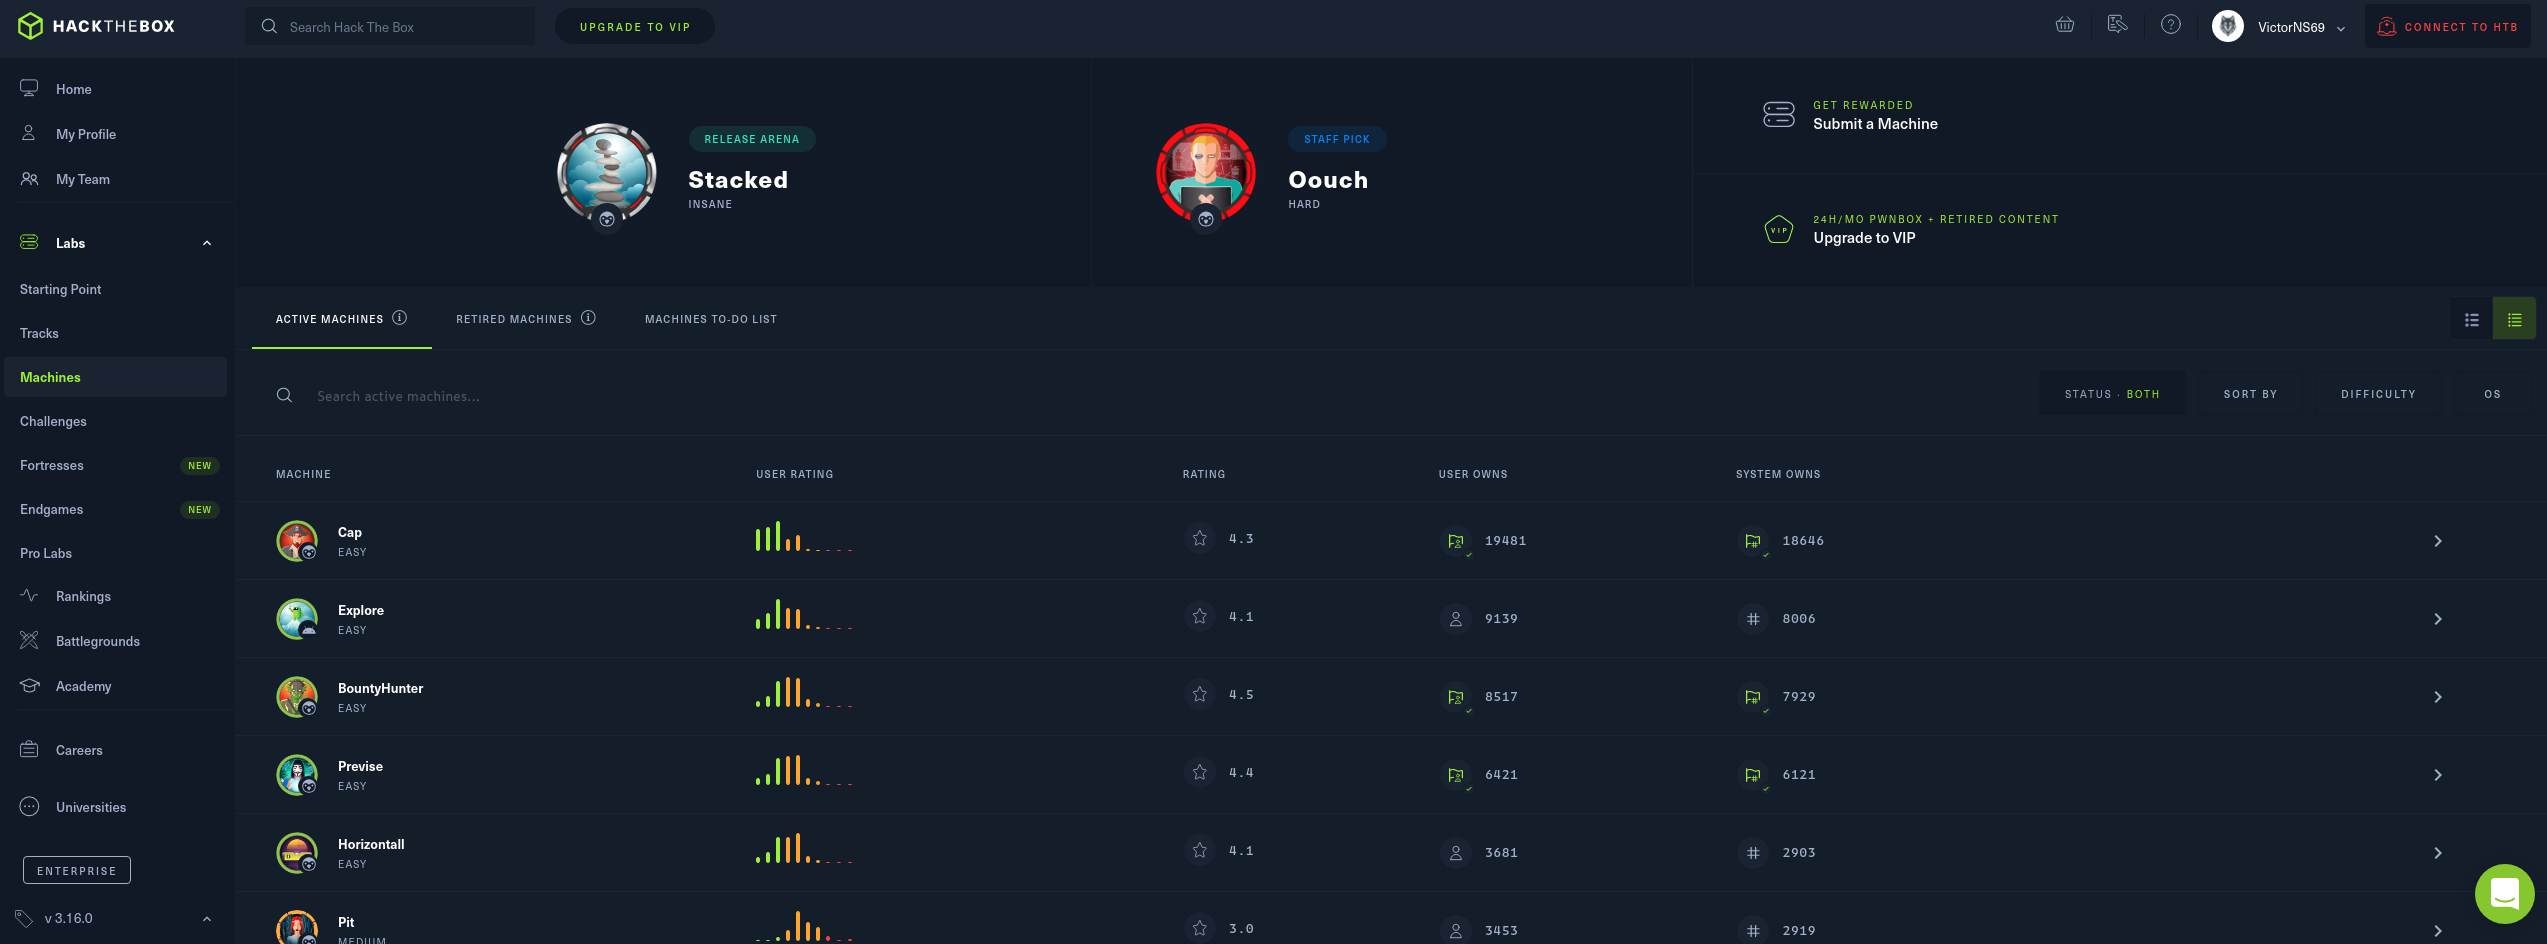
\includegraphics[width=1.0\textwidth]{images/sections/stateOfTheArt/htb-machines.png}
    \caption{\textit{Machines} en \textit{\acrshort{HTB}}}
    \label{fig:htb-machines}
\end{figure}

\subsubsection{Tracks}
Un \textit{Track} es un conjunto de máquinas y desafíos enlazados entre sí, centradas en un objetivo o tecnología concreta, que permite al usuario profundizar sobre ese tema en concreto. En la siguiente figura (figura \ref{fig:htb-tracks}) se puede ver el primer \textit{track} disponible.
\begin{figure}[h]
    \centering
    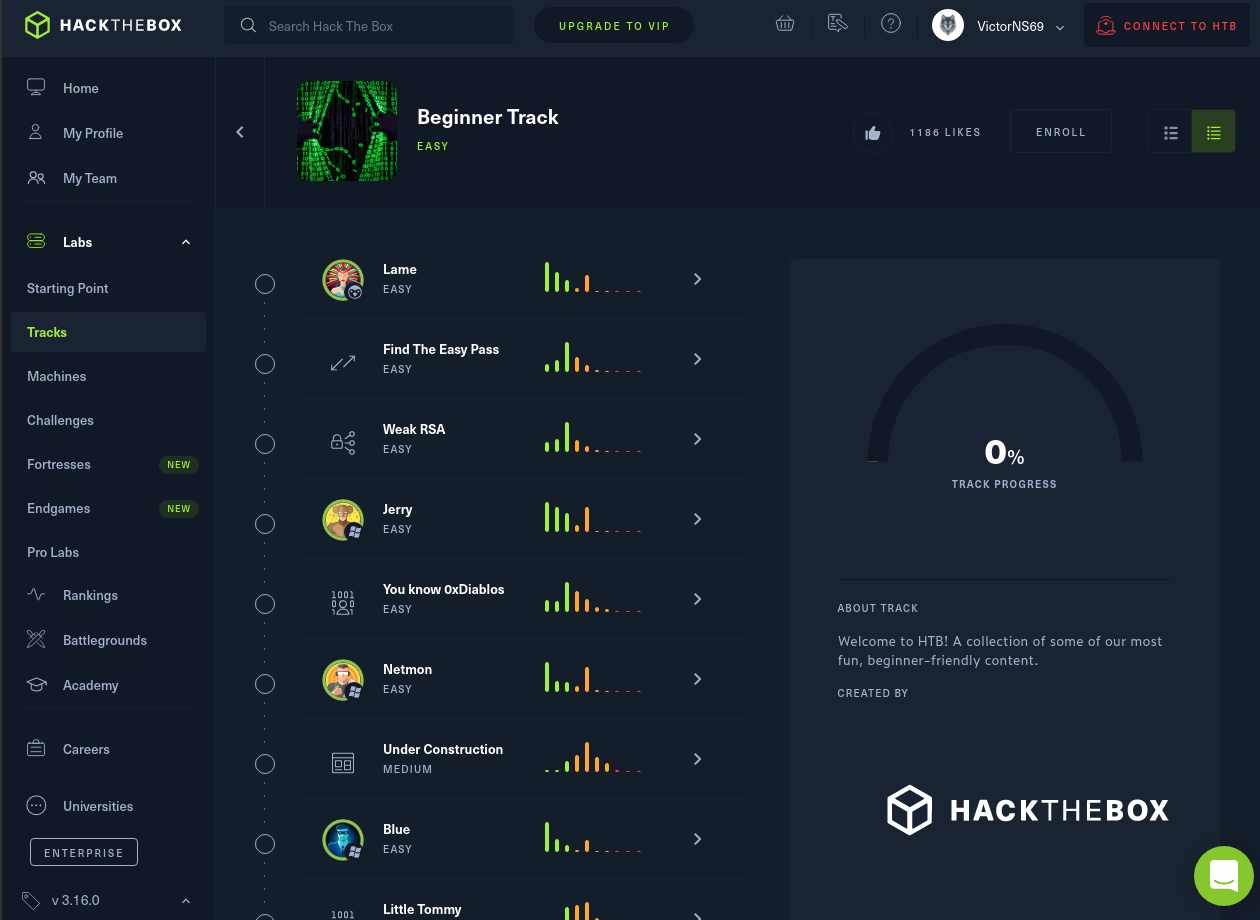
\includegraphics[width=0.6\textwidth]{images/sections/stateOfTheArt/htb-tracks.png}
    \caption{\textit{Beginner Track} en \textit{\acrshort{HTB}}}
    \label{fig:htb-tracks}
\end{figure}

\subsubsection{Endgames}
La sección \textit{endgames} de \acrshort{HTB} son una serie de laboratorios avanzados simulando escenarios e infraestructuras del mundo real. El objetivo, al igual que con las \textit{machines} es obtener el flag de \textit{root}, pero en estos laboratorios hay más máquinas, redes más complejas y un desafío mucho mayor.\\

Para desbloquear el \textit{endgame}, se tiene que haber alcanzado un rango mínimo en \acrshort{HTB} de ``\textit{Guru}``. El rango se consigue realizando máquinas, desafíos y demás.


    \subsection{\acrlong{CTF}}
    \input{sections/stateOfTheArt/ctf}

    \newpage
    \section{Herramientas}
    En esta sección se hablará de las distintas herramientas utilizadas a lo largo de todo el documento.

    \subsection{Anew}
    \textit{anew}\cite{anew} es una herramienta escrita en \textit{Golang} que añade las líneas que salen por la salida estándar de un comando a un archivo concreto, pero solo si esas líneas no estaban ya contenidas en el archivo. También imprime en la salida estándar las nuevas líneas que se han añadido, funcionando de manera similar a como \texttt{tee -a} eliminando los duplicados.\\

Un ejemplo de su uso se muestra en la figura \ref{fig:anew-example}. En el ejemplo se tiene una lista inicial con el contenido ``\textit{uno}``, ``\textit{dos}`` y ``\textit{tres}``, y una segunda lista con más números: ``\textit{dos}``, ``\textit{tres}``, ``\textit{cuatro}`` y ``\textit{cinco}``. Ejecutando el comando \textit{anew} entre las dos listas, obtenemos como resultado los valores de la segunda lista que no están en la primera (``\textit{cuatro}`` y ``\textit{cinco}``), además de actualizar la primera lista con dichos valores.

\begin{figure}[h]
    \centering
    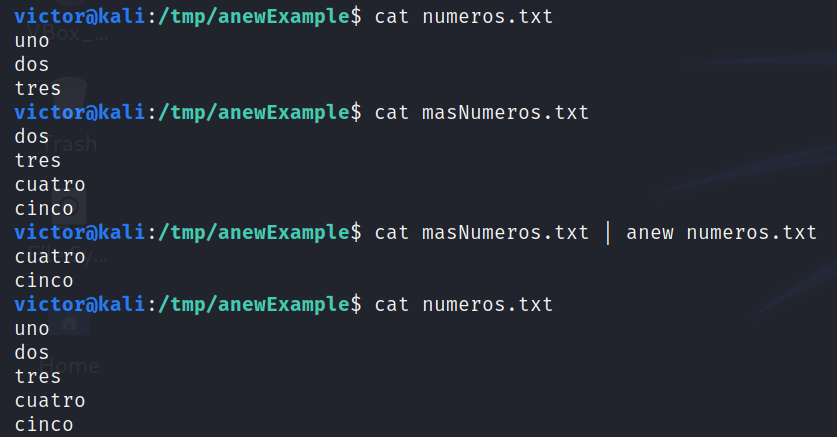
\includegraphics[width=0.80\textwidth]{images/sections/tools/anew-example.png}
    \caption{Ejemplo de uso de \textit{anew}}
    \label{fig:anew-example}
\end{figure}

    \subsection{Gobuster}
    \textit{Gobuster}\cite{gobuster} es una herramienta escrita en \textit{Golang} utilizada para realizar fuerza bruta en \acrshort{uri}s, en \acrshort{dns}, en servidores web y en \textit{buckets} de \textit{Amazon S3}.\\

\textit{Gobuster} destaca por tener varios modos de escaneo.

\begin{itemize}
    \item Modo \texttt{\textbf{dir}}: el modo clásico de escaneo de directorios mediante fuerza bruta.
    \item Modo \texttt{\textbf{dns}}: modo de fuerza bruta mediante subdominios \acrshort{dns}.
    \item Modo \texttt{\textbf{fuzz}}: utilizado para hacer \textit{fuzzing}.
    \item Modo \texttt{\textbf{s3}}: enumera \textit{buckets S3} abiertos y mira por la existencia de listados de \textit{buckets}.
    \item Modo \texttt{\textbf{vhost}}: fuerza bruta mediante hosts virtuales.
\end{itemize}

\textit{Gobuster} tiene varias opciones para su uso, como se muestra en la figura \ref{fig:gobuster-help}, además de aún más opciones dependiendo del modo de uso elegido.\\

\begin{figure}[h]
    \centering
    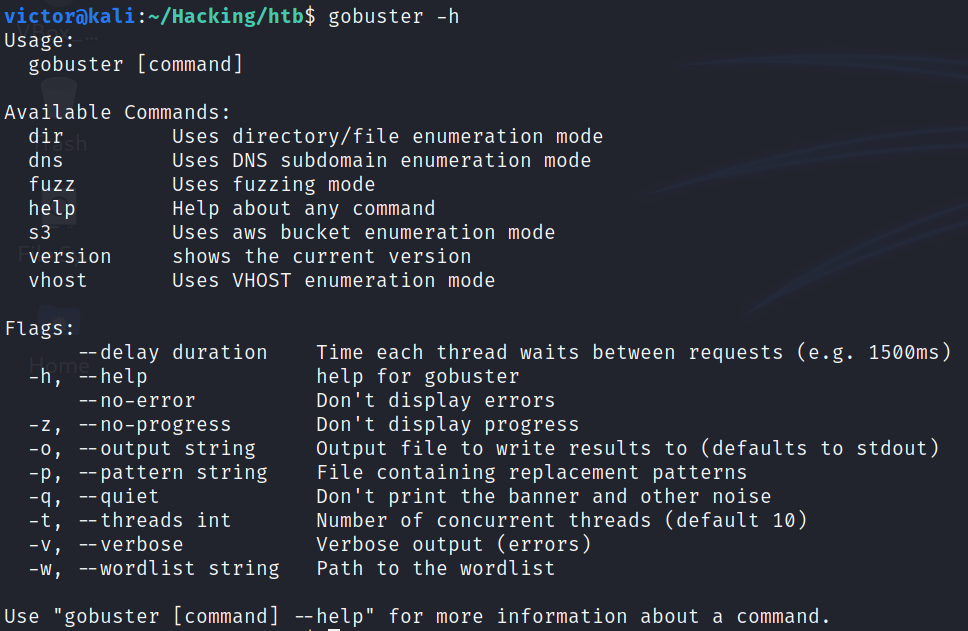
\includegraphics[width=0.7\textwidth]{images/sections/tools/gobuster.png}
    \caption{Ayuda de general de \textit{Gobuster}}
    \label{fig:gobuster-help}
\end{figure}

Algunos ejemplos de su uso son:

\begin{lstlisting}[language=bash]
gobuster dir -u https://mysite.com/path/to/folder -c 'session=123456' -t 50 -w common-files.txt -x .php,.html
gobuster dns -d mysite.com -t 50 -w common-names.txt
gobuster fuzz -u https://example.com?FUZZ=test -w parameter-names.txt
\end{lstlisting}

    \subsection{Nmap}
    \textit{Network Mapper} mayormente conocido como \textit{Nmap}\cite{nmap} es una herramienta gratuita y open source. Esta herramienta es usada para descubrimiento de red y auditorías de seguridad, además, muchos administradores de red utilizan esta herramienta para realizar tareas como inventario de red, gestionar los horarios de actualización de los servicios y monitorizar el \textit{uptime} de los servicios.\\

\textit{Nmap} utiliza paquetes \acrshort{ip} sin procesar de diversas maneras para determinar máquinas disponibles en la red, los servicios que dichas máquinas están exponiendo a la red, el sistema operativo, y docenas de otras características.\\

\textit{Nmap} destaca por:

\begin{itemize}
    \item Su \textbf{potencia}: puede escanear grandes redes de miles de máquinas.
    \item \textbf{Portabilidad}: es soportado por la mayoría de sistemas operativos, incluyendo \textit{Linux}, \textit{Windows} y \textit{Mac OS X}.
    \item Fácil \textbf{usabilidad}: pese a su gran cantidad de opciones, con tan solo escribir \texttt{nmap -v -A target} podríamos escanear una red.
    \item Ser gratuito.
    \item \textbf{Documentación}: tiene una gran cantidad de opciones y características, todas ellas bien documentadas tanto en su web como los manuales\footnote{\href{https://linux.die.net/man/1/nmap}{Manual de \textit{Nmap}}} de uso.
    \item Ser apoyado por una gran \textbf{comunidad}.
    \item \textbf{Popular}: miles de personas descargan y utilizan \textit{Nmap} diariamente.
\end{itemize}

\textit{Nmap} tiene muchas opciones de uso, como se puede ver en la figura \ref{fig:nmap-help} (no se muestran todas las opciones por su longitud). Estas funcionalidades se pueden catalogar en:

\begin{itemize}
    \item Especificación del objetivo/s (\textit{target/s}).
    \item Descubrimiento de hosts.
    \item Técnicas de escaneo.
    \item Especificación y orden de escaneo de puertos.
    \item Escaneo con scripts.
    \item Detección de sistema operativo.
    \item Temporización y rendimiento.
    \item Evasión de Firewall/\acrshort{ids} y \textit{Spoofing}.
    \item Gestión de la salida del comando.
    \item Miscelánea.
\end{itemize}

\begin{figure}[h]
    \centering
    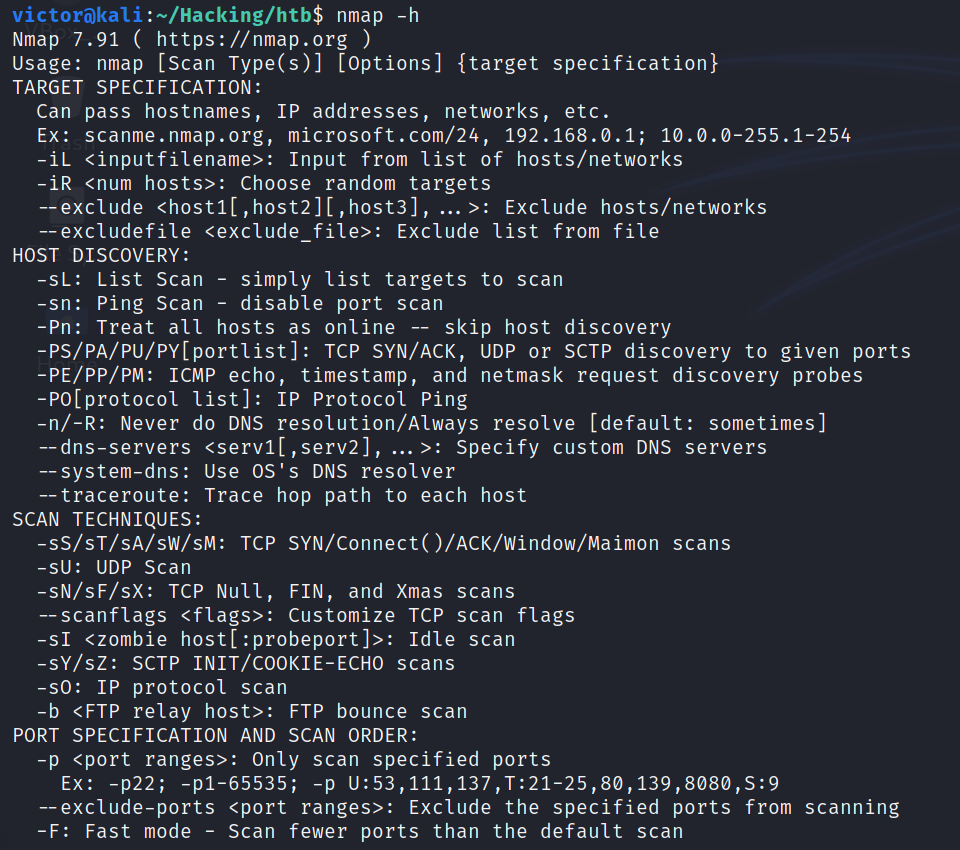
\includegraphics[width=0.65\textwidth]{images/sections/tools/nmap-help.png}
    \caption{Parte de la ayuda de \textit{Nmap}}
    \label{fig:nmap-help}
\end{figure}

Algunos ejemplos de uso son:

\begin{lstlisting}[language=bash]
nmap -v -A scanme.nmap.org
nmap -v -sn 192.168.0.0/16 10.0.0.0/8
nmap -v -iR 10000 -Pn -p 80
\end{lstlisting}

    \subsection{PEASS-ng}
    \textit{PEASS}\cite{peas} (figura \ref{fig:peass-logo}) son las siglas de \textit{Privilege Escalation Awesome Scripts}. \textit{PEASS} es un conjunto de herramientas utilizadas para la escalada de privilegios en los sistemas \textit{Windows}, \textit{Linux/Unix} y \textit{Mac OS}. Estas herramientas buscan por posibles caminos para la escalada de privilegios local que se puedan explotar. El resultado los imprime con diversos colores para que se puedan visualizar de manera sencilla las distintas fallas de configuración.\\

\begin{figure}[h]
    \centering
    
\includegraphics[width=0.35\textwidth]{images/sections/tools/peass.png}
    \caption{Logo de \textit{PEASS-ng}}
    \label{fig:peass-logo}
\end{figure}

Se denomina \textit{\textbf{WinPEAS}}\footnote{\href{https://github.com/carlospolop/PEASS-ng/tree/master/winPEAS}{Web de \textit{WinPEAS}}} a las herramientas utilizadas para la escalada de privilegios en sistemas \textit{Windows}. Los scripts para \textit{Windows} se pueden encontrar en formato \texttt{.exe} y \texttt{.bat}.\\

\textit{\textbf{LinPEASS}}\footnote{\href{https://github.com/carlospolop/PEASS-ng/tree/master/linPEAS}{Web de \textit{LinPEAS}}} es el script utilizado para la escalada de privilegios en sistemas \textit{Linux/Unix} y \textit{Mac OS} (automáticamente el script detecta si es un sistema \textit{Mac}). Como se puede ver en la siguiente figura (figura \ref{fig:linpeas-help}), \textit{linPEAS} tiene diversas opciones para su uso.

\begin{figure}[h]
    \centering
    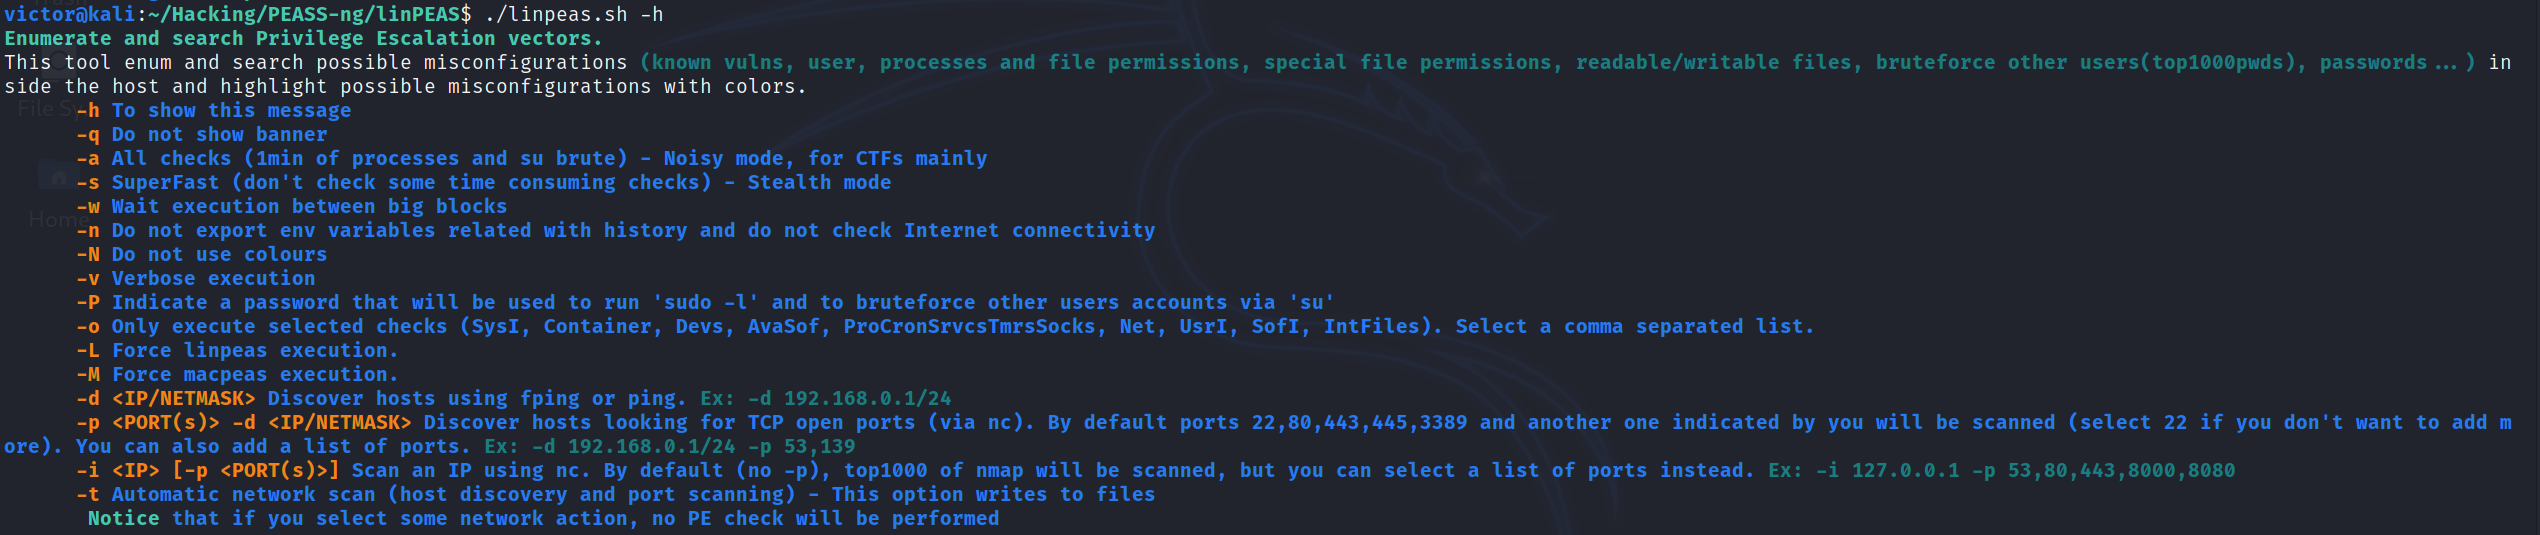
\includegraphics[width=1.0\textwidth]{images/sections/tools/linpeas-help.png}
    \caption{Ayuda \textit{linPEAS}}
    \label{fig:linpeas-help}
\end{figure}

A continuación se muestra un extracto de la salida del script (figura \ref{fig:linpeas-out}).

\begin{figure}[h]
    \centering
    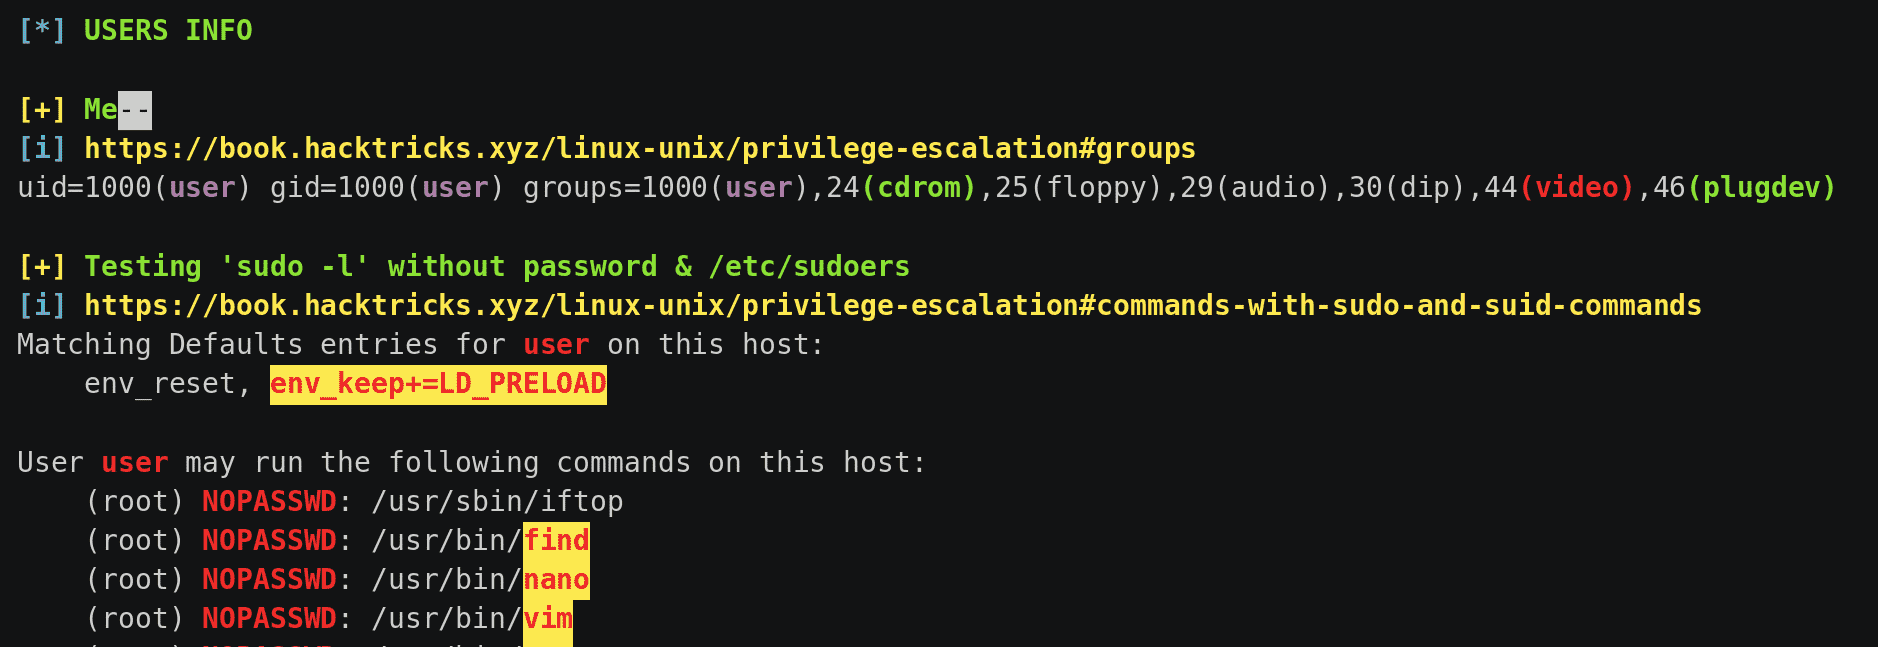
\includegraphics[width=1.0\textwidth]{images/sections/tools/linpeas-out.png}
    \caption{Extracto de la salida de \textit{linPEAS}}
    \label{fig:linpeas-out}
\end{figure}

    \subsection{SecLists}
    \textit{SecLists}\cite{seclists} es una colección de múltiples tipos de listas usadas en durante los análisis de seguridad. Entre las listas se incluyen nombres de usuarios, contraseñas, \acrshort{url}s, patrones de información sensible, payloads para fuzzing y más.\\

El directorio cuenta en actualidad con un tamaño de 2.5 GB y más de 5400 listas.

    \subsection{Wireshark}
    \textit{Wireshark}\cite{wireshark} (figura \ref{fig:wire-logo}) es el analizador de tráfico de red más importante y más utilizado. \textit{Wireshark} permite observar el trafico de red en tiempo real y lo muestra en un formato legible para las personas. Cuenta con una gran cantidad de filtros y características, como detectar rápidamente problemas de red como latencia, actividad sospechosa y paquetes caídos. También puede profundizar en el tráfico y descubrir la causa raíz de un problema. Por lo general, los administradores de red usan \textit{Wireshark} para resolver los problemas de latencia causados por los equipos utilizados para enrutar el tráfico alrededor del mundo y para monitorizar los intentos de exfiltración de datos en las operaciones comerciales.\\

\begin{figure}[h]
    \centering
    
\includegraphics[width=0.30\textwidth]{images/sections/tools/wireshark-logo.png}
    \caption{Logo de \textit{Wireshark}}
    \label{fig:wire-logo}
\end{figure}

\textit{Wireshark} consta de un amplio conjunto de funciones que incluye lo siguiente:

\begin{itemize}
    \item Captura en vivo y permite análisis fuera de línea
    \item Análisis completo de \acrshort{voip}
    \item Permite leer/escribir en muchos formatos de archivo de captura diferentes
    \item Captura archivos comprimidos y descomprímalos sobre la marcha
    \item Inspecciona profundamente cientos de protocolos
    \item Utiliza una interfaz de usuario cómoda e intuitiva
    \item Funciona en \textit{Linux}, \textit{Windows}, \textit{Mac OS X} y \textit{FreeBSD}
    \item Tiene potentes filtros de visualización
    \item La salida se puede exportar a \textit{XML}, \textit{CSV}, \textit{PostScript} o como texto sin formato
\end{itemize}

En la siguiente figura (figura \ref{fig:wire-example}), se puede ver un ejemplo de captura de red.

\begin{figure}[h]
    \centering
    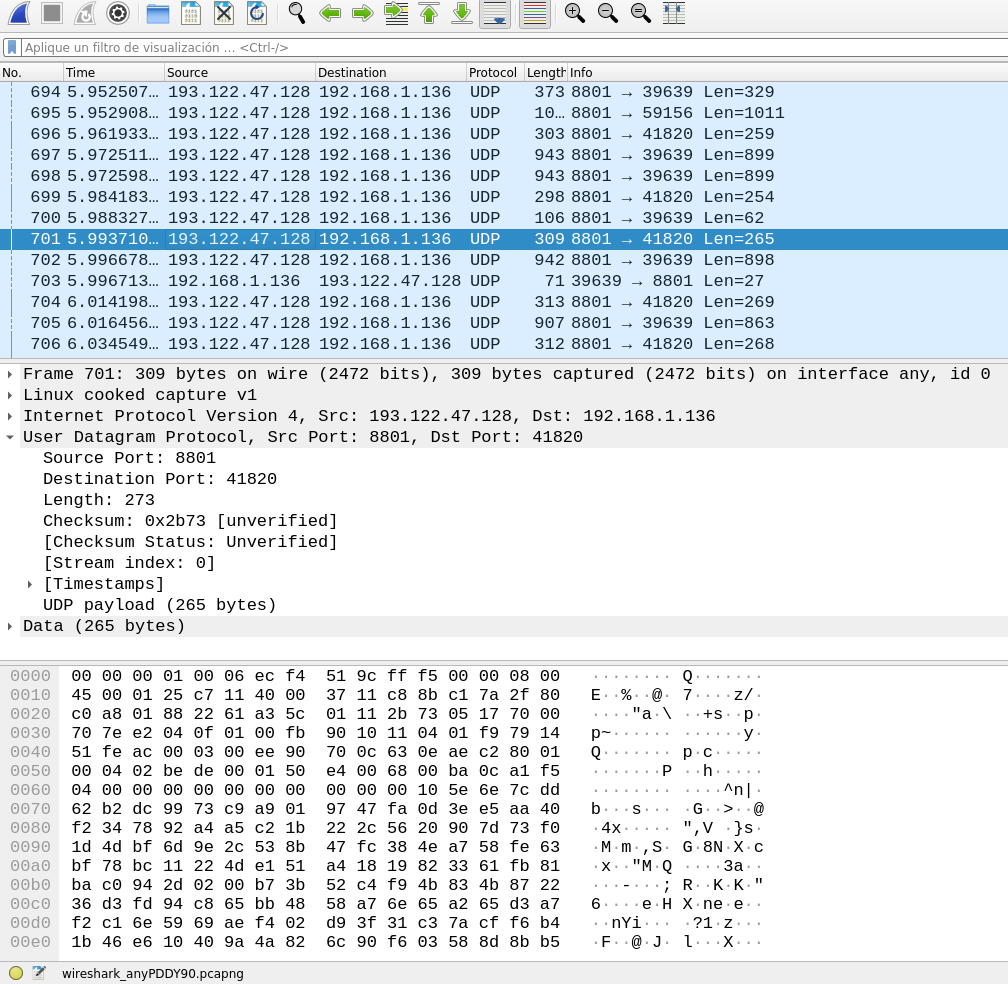
\includegraphics[width=1.0\textwidth]{images/sections/tools/wire-example.png}
    \caption{Captura de red con \textit{Wireshark}}
    \label{fig:wire-example}
\end{figure}


    \newpage
    \section{\acrshort{CTF} 1: \textit{Cap}}
    Esta sección se realizará la máquina de \acrlong{htb} llamada \textit{Cap}\cite{cap}. \textit{Cap} es una máquina de dificultad ``fácil``.

\subsection{Reconocimiento}
En la fase de reconocimiento hemos encontrado la información de la máquina en la propia página principal\cite{cap} de la misma. Se ha encontrado que es una máquina \textit{Linux} y que su IP es \texttt{10.10.10.245}.\\

Dado que es un \acrshort{CTF}, no se ha visto la necesidad de indagar más en esta fase.

\subsection{Enumeración}
El primer paso realizado en la enumeración es usar la herramienta \textit{Nmap}\cite{nmap}. Para ello se ha utilizado el siguiente comando.
\begin{lstlisting}[language=bash]
nmap -p- --min-rate 10000 -o 00_nmap_ports.txt 10.10.10.245
\end{lstlisting}
El argumento \texttt{-p-} para hacer un escaneo de todos los puertos; \texttt{--min-rate 10000} se ha utilizado para indicar a \textit{Nmap} que como mínimo envíe 10000 paquetes por segundo; por último, el argumento \texttt{-o ports.txt}, que es utilizado para guardar la salida en un archivo llamado \textit{00\_nmap\_ports.txt}.\\

Tras la ejecución del comando, se han encontrado los puertos 21/\acrshort{tcp}, 22/\acrshort{tcp} y 80/\acrshort{tcp} abiertos. Con este resultado\footnote{\href{https://github.com/VictorNS69/TFM/blob/main/machines/cap/00_nmap_ports.txt}{Output de \textit{00\_nmap\_ports.txt}}}, de nuevo ejecutamos \textit{Nmap} para sacar información sobre los servicios que se están ejecutando en cada puerto.\\

Se ha utilizado el siguiente comando:
\begin{lstlisting}[language=bash]
sudo nmap -p 21,22,80 -sS -sCV 10.10.10.245 -o 01_nmap_services.txt
\end{lstlisting}

Esta vez, el comando \texttt{-p} recibe los puertos obtenidos con el comando anterior, es decir, los puertos 21, 22 y 80 \acrshort{tcp}. Se ha decidido hacer un escaneo de tipo \textit{Stealth}, ya que es la manera más rápida y popular para escanear en el protocolo TCP; para ello se ha utilizado el argumento \texttt{-sS}. Se ha utilizado el comando \texttt{-sCV} para obtener información sobre el servicio habilitado en el puerto (\texttt{-sV}) y para realizar el escaneo con los scripts por defecto de \textit{Nmap} (\texttt{-sC}). Por último, también se ha decidido guardar la salida del comando en un archivo (argumento \texttt{-o} llamado \textit{01\_nmap\_services}.txt.\\

Tras la ejecución\footnote{\href{https://github.com/VictorNS69/TFM/blob/main/machines/cap/01_nmap_services.txt}{Output de \textit{01\_nmap\_services.txt}}} se ha encontrado que, efectivamente, la máquina es un sistema \textit{Linux}, concretamente con el sistema operativo \textit{Ubuntu}. Como era de esperar, en el puerto 21/\acrshort{tcp} se ha encontrado un servidor \acrshort{ftp}, está corriendo \textit{vsftpd}\cite{vsftpd} en la versión 3.0.3. En el puerto 22/\acrshort{tcp} está levantado un servidor \acrshort{ssh}, está utilizando \textit{OpenSSH}\cite{openssh} versión 8.2p1. Por último, en el puerto 80/\acrshort{tcp} un servidor \acrshort{http} \textit{Gunicorn}\cite{gunicorn}.\\

En este fase, también se ha decidido utilizar la herramienta \textit{Gobuster}\cite{gobuster} en la web, para encontrar endpoints no accesibles a primera vista. Para ello, se ha utilizado el siguiente comando:
\begin{lstlisting}[language=bash]
gobuster dir -u http://10.10.10.245 -w ~/Hacking/SecLists/Discovery/Web-Content/raft-large-words.txt | anew 03_gobuster.txt
\end{lstlisting}
Se ha elegido el argumento \texttt{dir} para realizar una búsqueda de directorios mediante fuerza bruta; el flag \texttt{-u} es el utilizado para pasar la \acrshort{url} que vamos  a escanear; el argumento \texttt{-w} se utiliza para pasarle a \textit{Gobuster} una lista de palabras para utilizar. En este caso se ha decidido usar la lista \textit{raft-large-words.txt} de \textit{SecLists}\cite{seclists}. Por último, el resultado de \textit{Gobuster} se ha decidido pasar a la herramienta \textit{anew}\cite{anew} porque también se ha realizado el mismo comando pero con la lista \textit{raft-large-directories.txt}.\\

Como resultado\footnote{\href{https://github.com/VictorNS69/TFM/blob/main/machines/cap/02_gobuster.txt}{Output de \textit{02\_gobuster.txt}}} se han encontrado las siguientes \acrshort{url}'s:
\begin{itemize}
    \item \texttt{/data}
    \item \texttt{/ip}
    \item \texttt{/capture} (redirecciona a \texttt{/data/16})
    \item \texttt{/netstat}
\end{itemize}

\subsection{Ganar acceso}

Lo primero que se ha intentado es acceder al servicio \acrshort{ssh} con contraseñas débiles, como \textit{admin:admin}, \textit{admin:Passw0rd} o \textit{admin:123456}, pero ninguna ha dado resultado.\\

Acto seguido se ha decidido investigar la web. Al abrir la página web (\texttt{http://10.\\10.10.245}), lo primero que encontramos es un dashboard (figura \ref{fig:cap}-a). Vemos que ya estamos logeados como \textit{Nathan}, y que algunos de los botones no funcionan, como \textit{Message} y \textit{Settings}.\\

También se ha investigado las pestañas del menú lateral izquierdo. Encontramos información de la red en los apartados \textit{IP Config} (figura \ref{fig:cap}-b) y \textit{Network Status} (figura \ref{fig:cap}-c).\\

\begin{figure}
    \centering
    \subfloat[\centering \textit{Cap: Dashboard (\texttt{http://10.10.10.245/})}]{{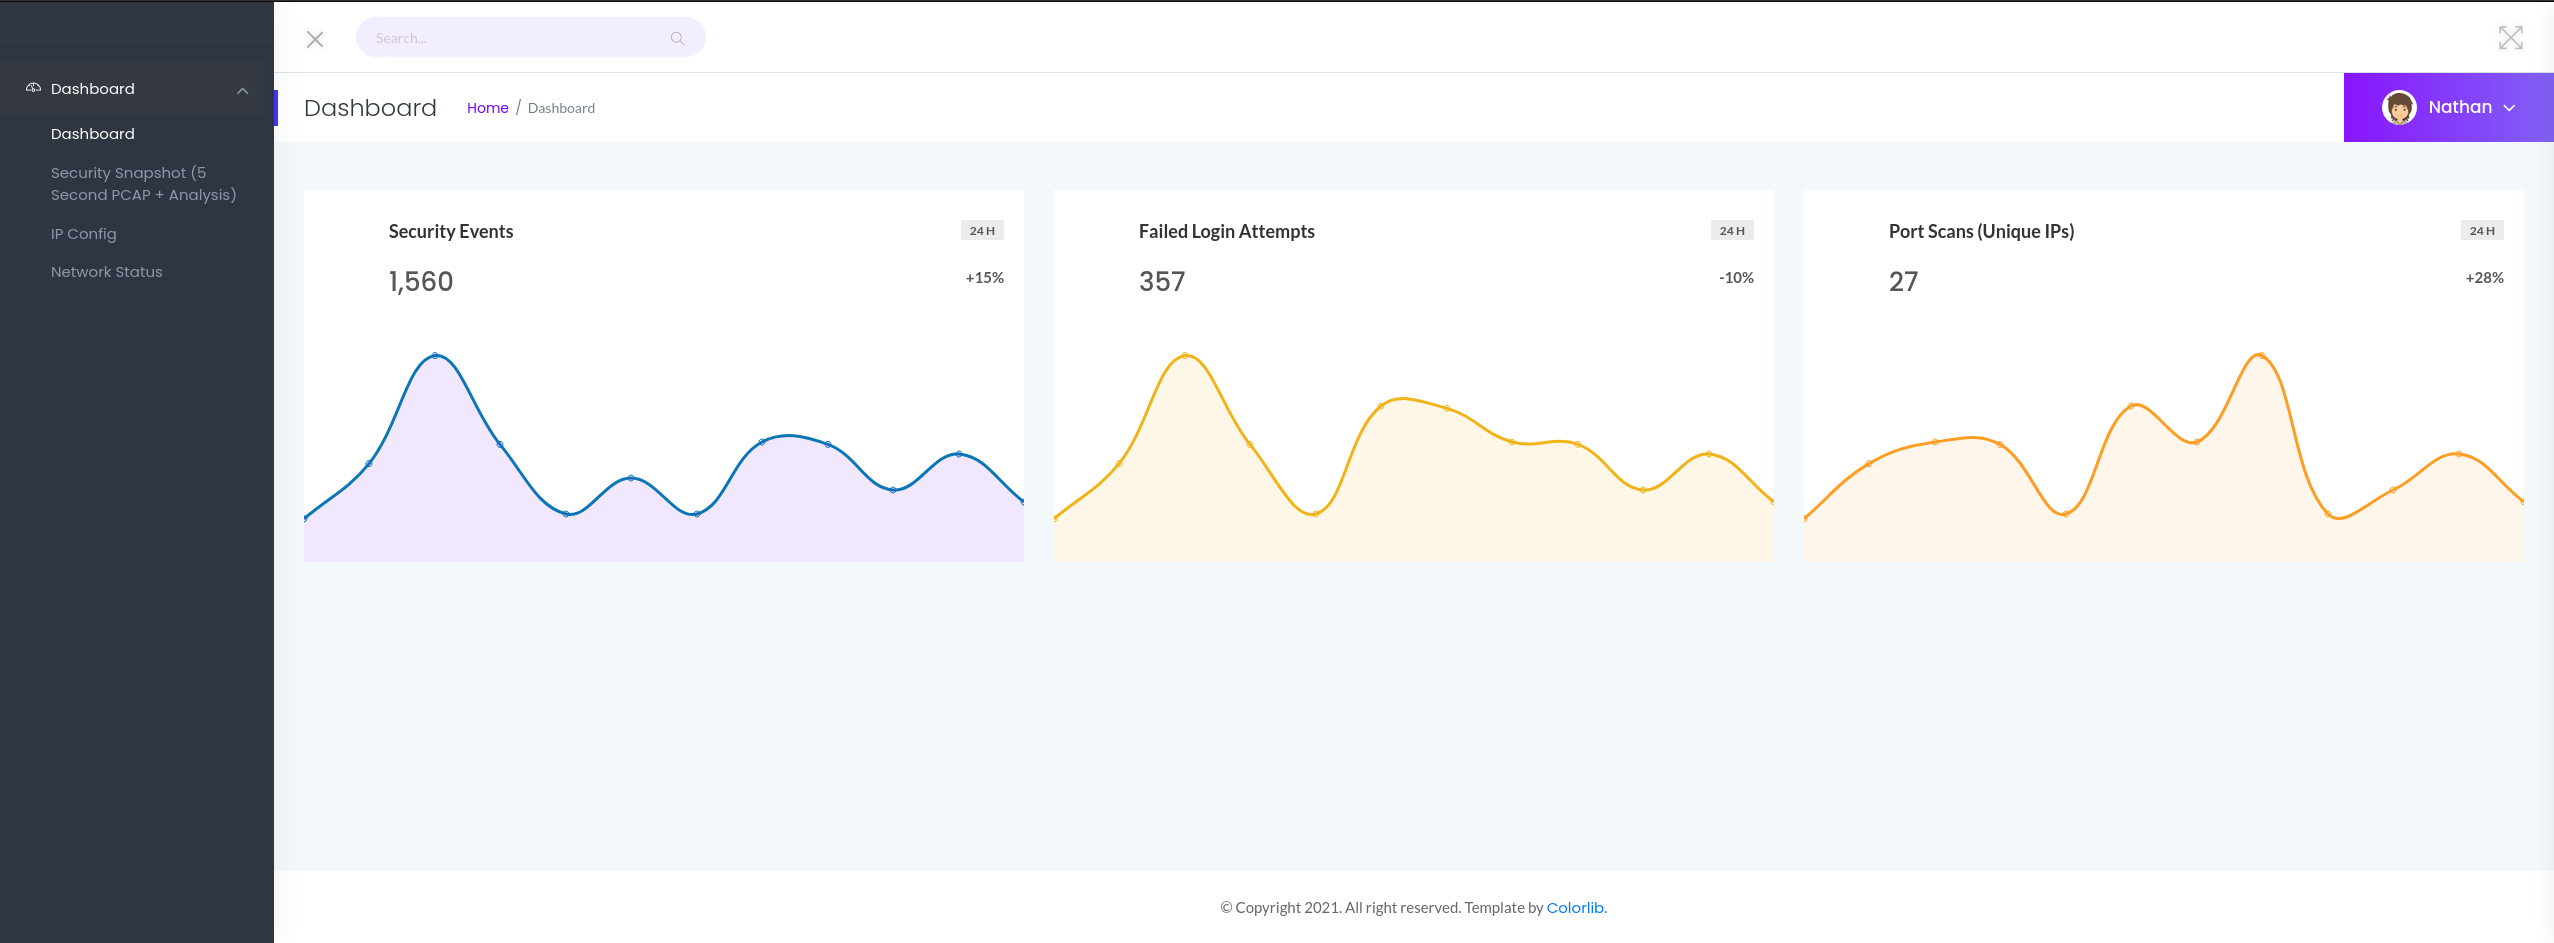
\includegraphics[width=0.80\textwidth]{images/machines/cap/web-dashboard.png} }}%
    \qquad
    \subfloat[\centering \textit{Cap: IP Config (\texttt{http://10.10.10.245/ip})}]{{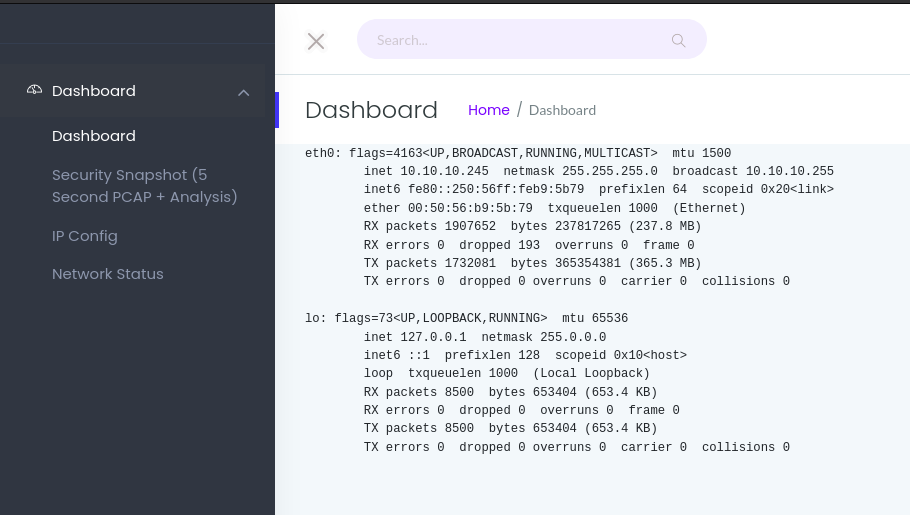
\includegraphics[width=0.80\textwidth]{images/machines/cap/web-ip.png} }}%
    \qquad
    \subfloat[\centering \textit{Cap: Network Status (\texttt{http://10.10.10.245/netstat})}]{{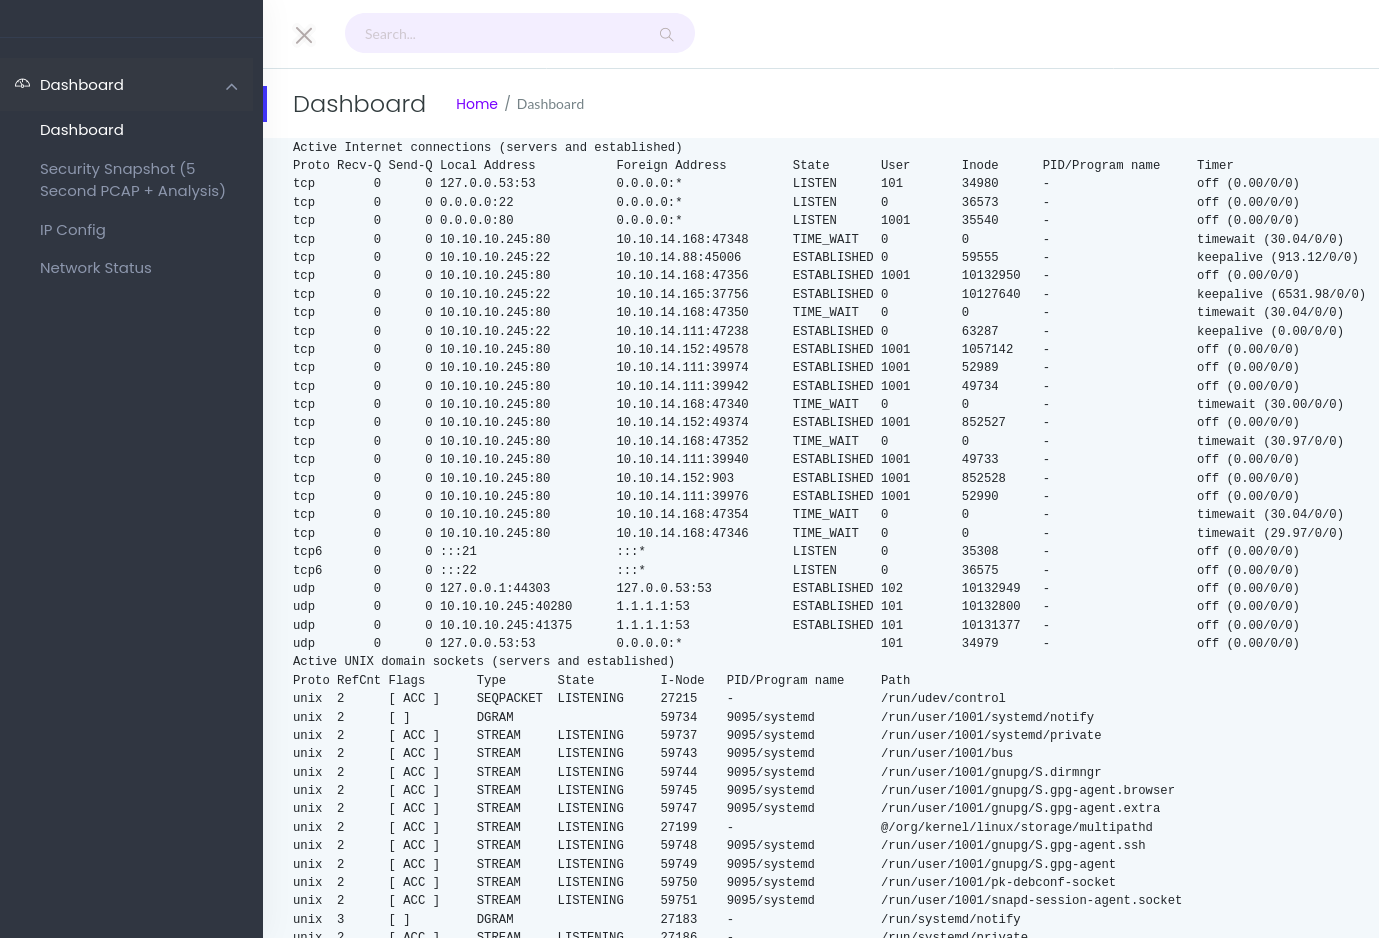
\includegraphics[width=0.80\textwidth]{images/machines/cap/web-network.png} }}
    \caption{Cap: Capturas de la web}
    \label{fig:cap}
\end{figure}

Por último, el apartado Security Snapshot (figura \ref{fig:cap-snapshot}) nos permite descargar un paquete \texttt{.pcap}. Al clicar el botón \textit{Download}, nos bajamos un archivo llamado \textit{16.pcap}\footnote{\href{https://github.com/VictorNS69/TFM/blob/main/machines/cap/pcaps/16.pcap}{Archivo \textit{16.pcap}}}. Nombre que coincide con la \acrshort{url}, ya que esta es \texttt{/data/16}. Investigamos el paquete con \textit{Wireshark}\cite{wireshark} (figura \ref{fig:cap-wire-16}).\\

\begin{figure}[h]
    \centering
    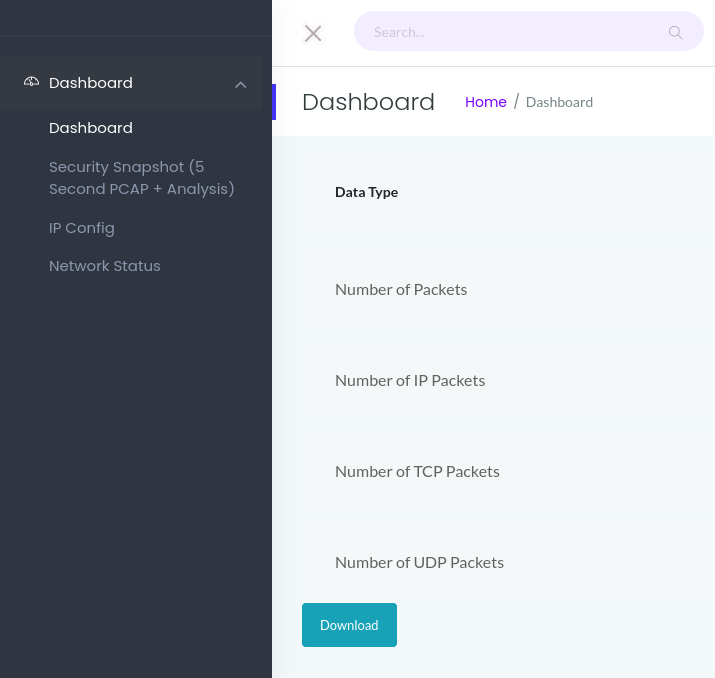
\includegraphics[width=0.40\textwidth]{images/machines/cap/web-sec-snapshots.png}
    \caption{Cap: Security Snapshot (\texttt{http://10.10.10.245/data/16})}
    \label{fig:cap-snapshot}
\end{figure}

\begin{figure}[h]
    \centering
    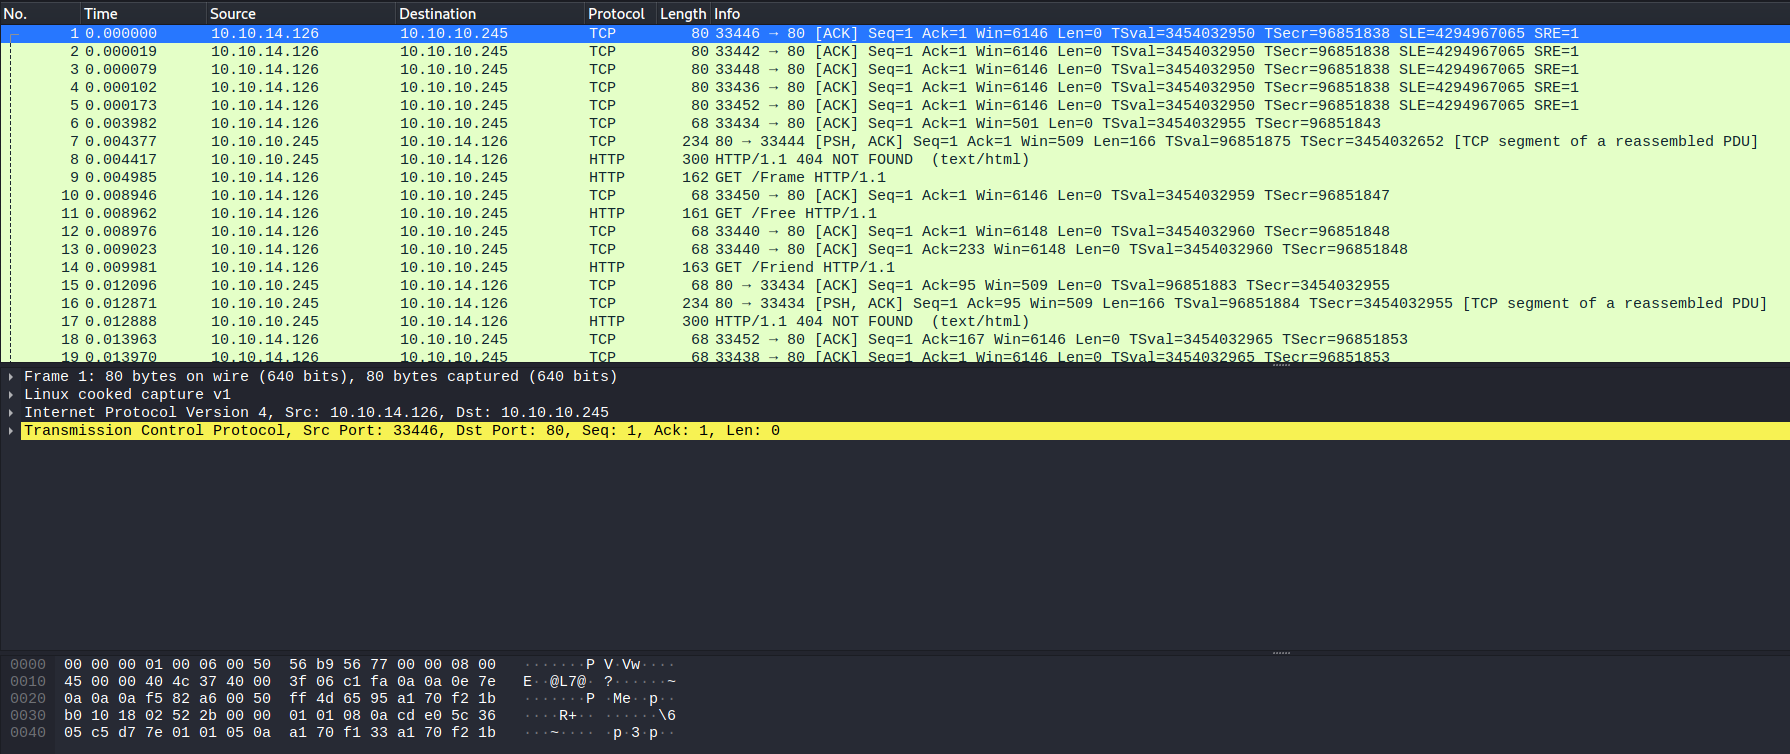
\includegraphics[width=1.0\textwidth]{images/machines/cap/wireshark-16.png}
    \caption{Archivo \textit{16.pcap} en \textit{Wireshark}}
    \label{fig:cap-wire-16}
\end{figure}

Tras investigar el archivo \texttt{16.pcap}, no se ha encontrado nada relevante. Tampoco se ha encontrado nada sobre los servicios \acrshort{ssh} y \acrshort{ftp}.\\

Al no encontrar nada en este paquete, se ha decidido probar con la \acrshort{url} \texttt{/data/\{?\}}. Se ha probado con los valores `0`, `1` y `1000`. En los casos `0` y `1` hemos conseguido entrar a \texttt{/data/0} y \texttt{/data/1} descargar los paquetes \texttt{0.pcap}\footnote{\href{https://github.com/VictorNS69/TFM/blob/main/machines/cap/pcaps/0.pcap}{Archivo \textit{0.pcap}}} y \texttt{1.pcap}\footnote{\href{https://github.com/VictorNS69/TFM/blob/main/machines/cap/pcaps/1.pcap}{Archivo \textit{1.pcap}}}, pero con el valor `1000` hemos sido redirigidos a la página principal.\\

Se ha decidido empezar por orden, y empezar revisando primero \texttt{0.pcap}. Al revisar el paquete, encontramos que en este hay movimiento en los puertos 21 y 22. Además, encontramos un inicio de sesión exitoso en el servidor \acrshort{ftp}. Como se ve en la figura \ref{fig:cap-wire-0}, se encuentran las credenciales \textit{nathan:Buck3tH4TF0RM3!}.\\
\begin{figure}[h]
    \centering
    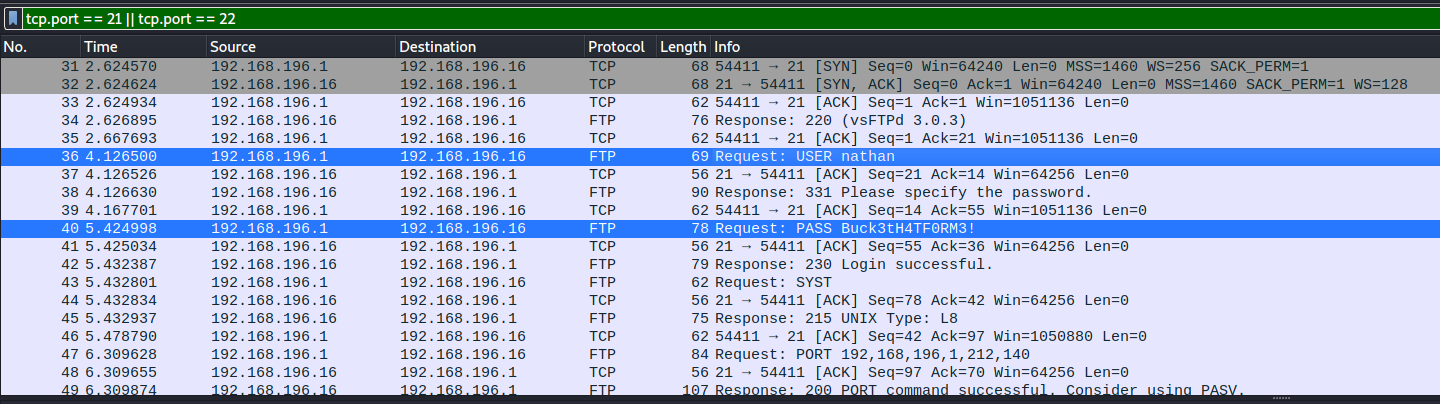
\includegraphics[width=1.0\textwidth]{images/machines/cap/wireshark-0.png}
    \caption{Archivo \textit{0.pcap} en \textit{Wireshark}}
    \label{fig:cap-wire-0}
\end{figure}

Con las credenciales obtenidas, entramos al servidor \acrshort{ftp}, y, como se ve en la figura \ref{fig:cap-user-flag}, obtenemos el flag de usuario.
\begin{figure}[h]
    \centering
    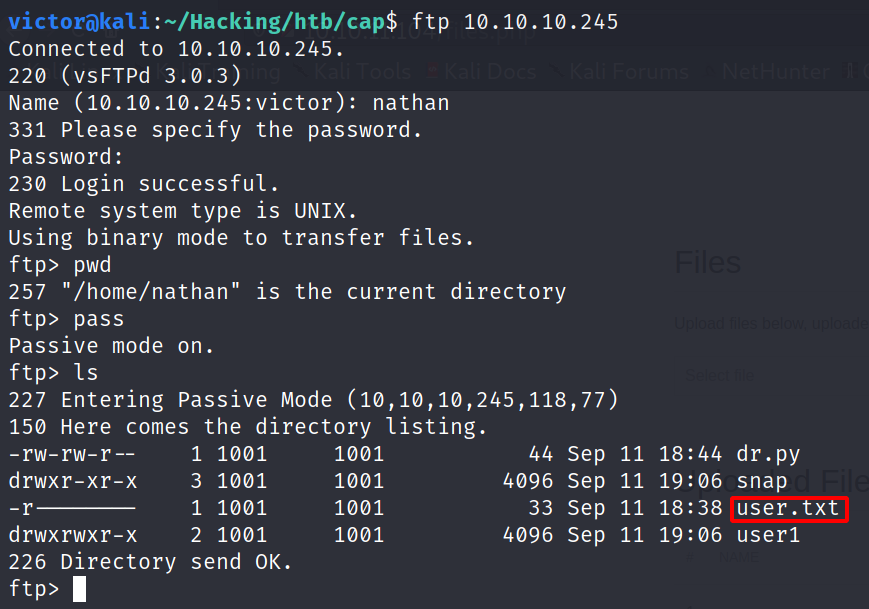
\includegraphics[width=0.8\textwidth]{images/machines/cap/user-flag.png}
    \caption{Acceso al servidor \acrshort{ftp} y obtención del flag de usuario}
    \label{fig:cap-user-flag}
\end{figure}

\subsection{Escalada de Privilegios}

Lo primero que se decide hacer es intentar acceder al \acrshort{ssh} con las credenciales anteriores. Conseguimos entrar.\\

Primero, intentamos ver si el usuario \textit{nathan} puede ejecutar algo como súper-usuario. Vemos que \textit{nathan} no puede usar \texttt{sudo} (figura \ref{fig:cap-nathan-sudo}). Para encontrar si el usuario \textit{nathan} puede ejecutar algún comando con permisos de súper-usuario, se ha utilizado la herramienta \textit{linPEAS}\cite{peas}. Para poder utilizar \textit{linPEAS}, tenemos que tener el script en la máquina víctima. Para pasar el script de nuestro host a la máquina, se ha utilizado el siguiente comando:
\begin{lstlisting}[language=bash]
scp ./linpeas.sh nathan@10.10.10.245:/home/nathan
\end{lstlisting}

\begin{figure}[h]
    \centering
    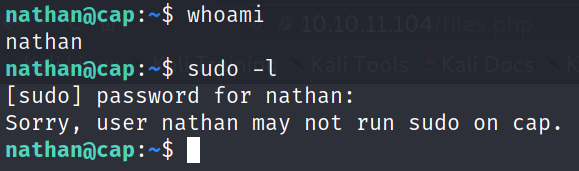
\includegraphics[width=0.5\textwidth]{images/machines/cap/nathan-sudo.png}
    \caption{Login \acrshort{ssh} con \textit{nathan} y comprobación de \texttt{sudo}}
    \label{fig:cap-nathan-sudo}
\end{figure}

Una vez subido el script, lo ejecutamos con:
\begin{lstlisting}[language=bash]
./linpeas.sh -a > 03_linpeas.txt
\end{lstlisting}

El flag \texttt{-a} es utilizado para revisar todos los checks posibles; es recomendado en la realización de un \acrshort{CTF}.\\

Como resultado\footnote{\href{https://github.com/VictorNS69/TFM/blob/main/machines/cap/03_linpeas.txt}{Output de \textit{03\_linpeas.txt}}} vemos que \textit{nathan} puede utilizar \texttt{/usr/bin/python3.8} como \textit{root} (figura \ref{fig:cap-linpeas}).\\

\begin{figure}[h]
    \centering
    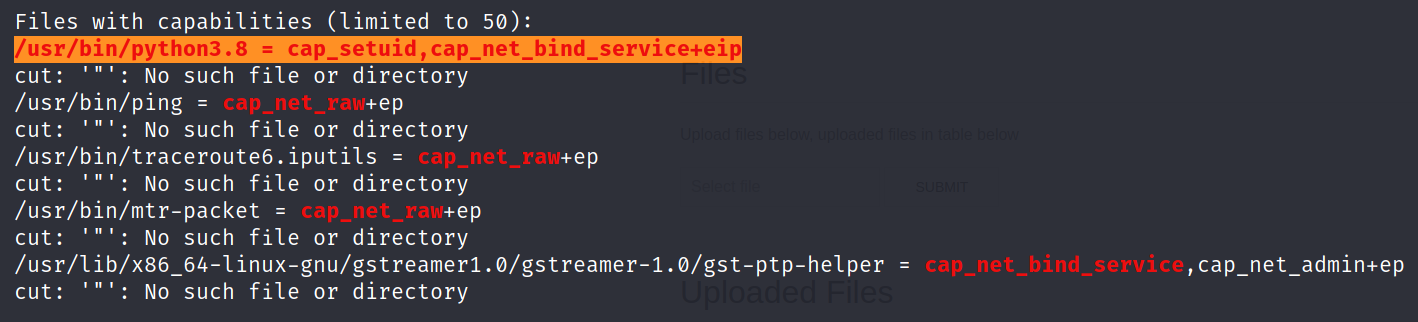
\includegraphics[width=1.0\textwidth]{images/machines/cap/linpeas.png}
    \caption{Resultado \textit{linPEAS}}
    \label{fig:cap-linpeas}
\end{figure}

Se ha investigado sobre posibles payloads y al final se ha decidido usar el siguiente para ganar acceso como \textit{root} (figura \ref{fig:cap-root}).
\begin{lstlisting}[language=bash]
python3 -c "import os; os.setuid(0); os.system('/bin/bash -i')"
\end{lstlisting}

\begin{figure}[h]
    \centering
    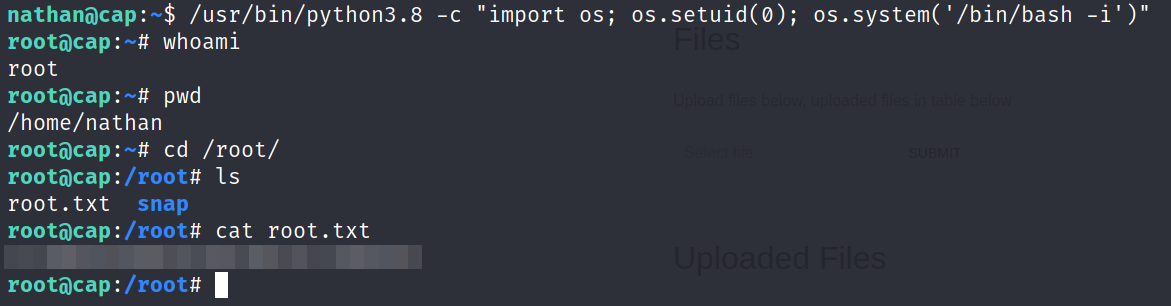
\includegraphics[width=0.8\textwidth]{images/machines/cap/root.png}
    \caption{Escalada de privilegios y obtención de \textit{root}}
    \label{fig:cap-root}
\end{figure}

\newpage

\subsection{Resumen}

En esta máquina hemos encontrado varias vulnerabilidades o malas prácticas. Por ejemplo, se han encontrado información sensible sobre la red y los además de los puertos abiertos en la máquina (figura \ref{fig:cap}). También se ha encontrado que, por una característica de la aplicación, te puedes bajar paquetes de esnifado de red (archivos \texttt{.pcap}). Esto sumado a que hay un servidor \acrshort{ftp} que no cifra las comunicaciones a la hora de iniciar sesión, nos ha podido encontrar las credenciales en claro en uno de los paquetes descargados. Esto nos ha permitido conectarnos al servidor \acrshort{ftp}. Además, se ha hecho uso de malas políticas de gestión de contraseñas y, se ha podido acceder al servicio \acrshort{ssh} con las mismas credenciales.\\

Una vez hemos entrado en la máquina vía \acrshort{ssh}, hemos podido subir un archivo (\texttt{linpeas.sh}) que nos ha permitido escanear la máquina, obteniendo así información sobre los permisos que tiene el usuario \textit{nathan}. Tras el escaneo, se ha encontrado que se puede ejecutar \textit{Python 3.8} como súper-usuario, lo cual, con un sencillo payload, nos permite acceder a la máquina como \textit{root}.

    \newpage
    \section{ctf2}

    \newpage
    \section{conclusiones}

    \newpage
    % \nocite{*} % Cita todas las ref (incluidas las no citadas)
    \printbibliography[heading=bibnumbered] % Última sección, numerada, para la bibliografía

\end{otherlanguage}
\end{document}
